 \thispagestyle{cackithitoannone}
\pagestyle{cackithitoan}
\everymath{\color{cackithi}}
\graphicspath{{../cackithi/pic/}}
%\blfootnote{{\color[named]{cackithi}$^1$Trường THPT chuyên Khoa học Tự nhiên, Đại học KHTN, Đại học Quốc Gia Hà Nội.}}
\begingroup
\AddToShipoutPicture*{\put(0,616){
\includegraphics[width=19.3cm]{../bannercackithi}}} 
\AddToShipoutPicture*{\put(108,525){
\includegraphics[scale=1]{../tieude.pdf}}} 
\centering
\endgroup
\vspace*{192pt}

\textit{\textbf{\color{cackithi}LTS.} Tạp chí Pi, tập $6$, số $7-8$, năm $2022$, đã giới thiệu với bạn đọc đôi nét về kỳ thi Olympic Toán của Pháp và đề bài của kỳ thi lần thứ $22$, năm $2022$. Trong số này, tạp chí Pi giới thiệu lời giải tóm tắt để bạn đọc tham khảo.}
\begin{multicols}{2}
	\textbf{\color{cackithi}Đề bài}
	\vskip 0.05cm
	\textbf{\color{cackithi}Bài $\pmb{1}$ (Chung cho tất cả thí sinh)}
	\vskip 0.05cm
	\textbf{\color{cackithi}Dán nhãn duyên dáng của một hình}
	\vskip 0.05cm
	Xét một tập hợp hữu hạn các điểm. Ta nối một số điểm trong số những điểm đã cho bởi những đoạn thẳng. Tập hợp được tạo ra theo cách đó được gọi là \textit{hình}.
	\vskip 0.05cm 
	Ta thực hiện việc \textit{dán nhãn} của một hình gồm $n$ đoạn thẳng bằng cách gắn mỗi đỉnh của hình đó với một số tự nhiên đôi một khác nhau trong khoảng từ $0$ tới $n$.
	\vskip 0.05cm 
	Mỗi đoạn thẳng được gán với giá trị tuyệt đối của hiệu giữa hai số tự nhiên được gắn cho hai đầu mút của đoạn thẳng đó. Giá trị tuyệt đối thu được là một số tự nhiên, được gọi là \textit{trọng số} của đoạn thẳng. 
	\vskip 0.05cm
	Ta nói rằng sự dán nhãn của một hình là \textit{duyên dáng} nếu $n$ trọng số nhận được trên các đoạn thẳng là những số tự nhiên từ $1$ tới~$n$.
	\vskip 0.05cm 
	Dưới đây là một ví dụ về sự dán nhãn duyên dáng cho một hình gồm $6$ điểm và $7$ đoạn thẳng.	
	\begin{figure}[H]
		\vspace*{-15pt}
		\centering
		\captionsetup{labelformat= empty, justification=centering}
		\begin{tikzpicture}[scale=0.78]
			\draw [cackithi,line width=0.8pt] (0.,2.)-- (4.,2.);
			\draw [cackithi,line width=0.8pt] (4.,2.)-- (4.,0.);
			\draw [cackithi,line width=0.8pt] (4.,0.)-- (0.,0.);
			\draw [cackithi,line width=0.8pt] (0.,0.)-- (0.,2.);
			\draw [cackithi,line width=0.8pt] (2.,2.)-- (2.,0.);
			
			\draw [fill=cackithi] (0.,2.) circle (2.5pt);
			\draw[color=cackithi] (-0.22,2.45) node {$0$};
			\draw [fill=cackithi] (4.,2.) circle (2.5pt);
			\draw[color=cackithi] (4.24,2.45) node {$2$};
			\draw [fill=cackithi] (4.,0.) circle (2.5pt);
			\draw[color=cackithi] (4.22,-0.4) node {$6$};
			\draw [fill=cackithi] (0.,0.) circle (2.5pt);
			\draw[color=cackithi] (-0.2,-0.4) node {$7$};
			\draw [fill=cackithi] (2.,2.) circle (2.5pt);
			\draw[color=cackithi] (2.,2.45) node {$3$};
			\draw [fill=cackithi] (2.,0.) circle (2.5pt);
			\draw[color=cackithi] (1.98,-0.4) node {$1$};
		\end{tikzpicture}
		
		\vspace*{-5pt}
		\caption{\small\textit{\color{cackithi}Hình được dán nhãn.}}
		\vspace*{-10pt}
	\end{figure}
	\begin{figure}[H]
		\vspace*{-10pt}
		\centering
		\captionsetup{labelformat= empty, justification=centering}
		\begin{tikzpicture}[scale=0.78]
			\draw [cackithi,line width=0.8pt] (0.,2.)-- (4.,2.);
			\draw [cackithi,line width=0.8pt] (4.,2.)-- (4.,0.);
			\draw [cackithi,line width=0.8pt] (4.,0.)-- (0.,0.);
			\draw [cackithi,line width=0.8pt] (0.,0.)-- (0.,2.);
			\draw [cackithi,line width=0.8pt] (2.,2.)-- (2.,0.);
			
			\draw [fill=cackithi] (0.,2.) circle (2.5pt);
			\draw[color=cackithi] (-0.22,2.45) node {$0$};
			\draw(1,2.5) node[squarednode]{$3$};
			\draw [fill=cackithi] (4.,2.) circle (2.5pt);
			\draw[color=cackithi] (4.24,2.45) node {$2$};
			\draw(3,2.5) node[squarednode]{$1$};
			\draw [fill=cackithi] (4.,0.) circle (2.5pt);
			\draw[color=cackithi] (4.22,-0.4) node {$6$};
			\draw(3,-0.5) node[squarednode]{$5$};
			\draw(1,-0.5) node[squarednode]{$6$};
			\draw(-0.5,1) node[squarednode]{$7$};
			\draw(1.5,1) node[squarednode]{$2$};
			\draw(4.5,1) node[squarednode]{$4$};
			\draw [fill=cackithi] (0.,0.) circle (2.5pt);
			\draw[color=cackithi] (-0.2,-0.4) node {$7$};
			\draw [fill=cackithi] (2.,2.) circle (2.5pt);
			\draw[color=cackithi] (2.,2.45) node {$3$};
			\draw [fill=cackithi] (2.,0.) circle (2.5pt);
			\draw[color=cackithi] (1.98,-0.4) node {$1$};
		\end{tikzpicture}
		
		\vspace*{-5pt}
		\caption{\small\textit{\color{cackithi}Hình được dán nhãn và trọng số.}}
		\vspace*{-10pt}
	\end{figure}
	\textbf{\color{cackithi}A. Một vài ví dụ}
	\vskip 0.05cm
	$1.$ Trong các hình dưới đây, hình nào cho ta một dán nhãn duyên dáng ?
	\begin{figure}[H]
		\vspace*{-15pt}
		\centering
		\captionsetup{labelformat= empty, justification=centering}
		\begin{tikzpicture}[scale=0.78]
			\draw [cackithi,line width=0.8pt] (0.,2.)-- (4.,2.);
			\draw [cackithi,line width=0.8pt] (4.,2.)-- (4.,0.);
			\draw [cackithi,line width=0.8pt] (4.,0.)-- (0.,0.);
			\draw [cackithi,line width=0.8pt] (0.,0.)-- (0.,2.);
			\draw [cackithi,line width=0.8pt] (2.,2.)-- (2.,0.);
			
			\draw [fill=cackithi] (0.,2.) circle (2.5pt);
			\draw[color=cackithi] (-0.22,2.45) node {$0$};
			\draw [fill=cackithi] (4.,2.) circle (2.5pt);
			\draw[color=cackithi] (4.24,2.45) node {$3$};
			\draw [fill=cackithi] (4.,0.) circle (2.5pt);
			\draw[color=cackithi] (4.22,-0.4) node {$5$};
			\draw [fill=cackithi] (0.,0.) circle (2.5pt);
			\draw[color=cackithi] (-0.2,-0.4) node {$7$};
			\draw [fill=cackithi] (2.,2.) circle (2.5pt);
			\draw[color=cackithi] (2.,2.45) node {$6$};
			\draw [fill=cackithi] (2.,0.) circle (2.5pt);
			\draw[color=cackithi] (1.98,-0.4) node {$1$};
		\end{tikzpicture}
		\vspace*{-10pt}
	\end{figure}
	\begin{figure}[H]
		\vspace*{-15pt}
		\centering
		\captionsetup{labelformat= empty, justification=centering}
		\begin{tikzpicture}[scale=0.78]
			\draw [cackithi, line width=0.8pt] (0.,2.)-- (4.,2.);
			\draw [cackithi,line width=0.8pt] (4.,2.)-- (4.,0.);
			\draw [cackithi,line width=0.8pt] (4.,0.)-- (0.,0.);
			\draw [cackithi,line width=0.8pt] (0.,0.)-- (0.,2.);
			\draw [cackithi,line width=0.8pt] (2.,2.)-- (2.,0.);
			
			\draw [fill=cackithi] (0.,2.) circle (2.5pt);
			\draw[color=cackithi] (-0.22,2.45) node {$0$};
			\draw [fill=cackithi] (4.,2.) circle (2.5pt);
			\draw[color=cackithi] (4.24,2.45) node {$2$};
			\draw [fill=cackithi] (4.,0.) circle (2.5pt);
			\draw[color=cackithi] (4.22,-0.4) node {$4$};
			\draw [fill=cackithi] (0.,0.) circle (2.5pt);
			\draw[color=cackithi] (-0.2,-0.4) node {$7$};
			\draw [fill=cackithi] (2.,2.) circle (2.5pt);
			\draw[color=cackithi] (2.,2.45) node {$7$};
			\draw [fill=cackithi] (2.,0.) circle (2.5pt);
			\draw[color=cackithi] (1.98,-0.4) node {$2$};
		\end{tikzpicture}
		\vspace*{-5pt}
	\end{figure}
	$2.$ Bổ sung hình sau để được một dán nhãn duyên dáng.
	\begin{figure}[H]
		\vspace*{-15pt}
		\centering
		\captionsetup{labelformat= empty, justification=centering}
		\begin{tikzpicture}[scale=0.85]
			\draw [cackithi,line width=0.75pt] (-1.6180339887498947,2.9021130325903073)-- (0.,2.38);
			\draw [cackithi,line width=0.8pt] (0.,2.38)-- (-1.,1.);
			\draw [cackithi,line width=0.8pt] (0.,2.38)-- (1.,1.);
			\draw [cackithi,line width=0.8pt] (0.,2.38)-- (1.618033988749895,2.9021130325903064);
			\draw [cackithi,line width=0.8pt] (0.,4.077683537175253)-- (0.,2.38);
			\draw [cackithi,line width=0.8pt] (0.,4.077683537175253)-- (-1.6180339887498947,2.9021130325903073);
			\draw [cackithi,line width=0.8pt] (-1.6180339887498947,2.9021130325903073)-- (-1.,1.);
			\draw [cackithi,line width=0.8pt] (-1.,1.)-- (1.,1.);
			\draw [cackithi,line width=0.8pt] (1.,1.)-- (1.618033988749895,2.9021130325903064);
			\draw [cackithi,line width=0.8pt] (1.618033988749895,2.9021130325903064)-- (0.,4.077683537175253);
			\draw [fill=cackithi] (-1.,1.) circle (2.5pt);
			%					\draw[color=cackithi] (-1.18624795654696,0.7809397247271022) node {$A$};
			\draw [fill=cackithi] (1.,1.) circle (2.5pt);
			%					\draw[color=cackithi] (1.209997363286399,0.7471897906449423) node {$B$};
			\draw [fill=cackithi] (1.618033988749895,2.9021130325903064) circle (2.5pt);
			\draw[color=cackithi] (1.8681210778885187,3.1434351104783014) node {$9$};
			\draw [fill=cackithi] (0.,4.077683537175253) circle (2.5pt);
			\draw[color=cackithi] (0.028749670410799504,4.4428075726414615) node {$4$};
			\draw [fill=cackithi] (-1.6180339887498947,2.9021130325903073) circle (2.5pt);
			\draw[color=cackithi] (-1.9624964404366394,3.0928102093550613) node {$10$};
			\draw [fill=cackithi] (0.,2.38) circle (2.5pt);
			\draw[color=cackithi] (-0.005000263671360479,2.012812318725942) node {$0$};
		\end{tikzpicture}
		\vspace*{-10pt}
	\end{figure}
	\textbf{\color{cackithi}B. Trường hợp thẳng hàng}
	\vskip 0.05cm
	Với mỗi số nguyên dương $n$, ta xét hình $L_n$ gồm $n+1$ điểm thẳng hàng và $n$ đoạn thẳng được tạo thành từ các điểm kề nhau.
	\vskip 0.05cm
	Ta đề xuất sự gán nhãn duyên dáng của những điểm của hình $L_4$ như sau :
	\begin{figure}[H]
		\vspace*{-10pt}
		\centering
		\captionsetup{labelformat= empty, justification=centering}
		\begin{tikzpicture}
			\draw[cackithi, line width=0.8pt] (0,0) -- (4,0);
			\draw [fill=cackithi] (0,0) node[above]{$0$} circle (2.5pt);
			\draw [fill=cackithi] (1,0) node[above]{$4$} circle (2.5pt);
			\draw [fill=cackithi] (2,0) node[above]{$1$} circle (2.5pt);
			\draw [fill=cackithi] (3,0) node[above]{$3$} circle (2.5pt);
			\draw [fill=cackithi] (4,0) node[above]{$2$} circle (2.5pt);
			
			\draw(0.5,-0.5) node[squarednode]{$4$};
			\draw(1.5,-0.5) node[squarednode]{$3$};
			\draw(2.5,-0.5) node[squarednode]{$2$};
			\draw(3.5,-0.5) node[squarednode]{$1$};
		\end{tikzpicture}
		\vspace*{-10pt}
	\end{figure}
	$1.$ Chứng minh rằng tồn tại một dán nhãn duyên dáng cho mỗi hình $L_5,L_6$ và $L_7$.
	\vskip 0.05cm
	$2.$ Ta chấp nhận mà không chứng minh rằng tồn tại một dán nhãn duyên dáng đối với hình $L_{2022}$ sao cho điểm ngoài cùng bên trái được gắn số $0$. Hãy mô tả sự dán nhãn này. 
	\vskip 0.05cm
	\textbf{\color{cackithi}C. Trường hợp đa giác}
	\vskip 0.05cm
	$1.$ Chứng minh rằng mọi tam giác và tứ giác đều có thể được dán nhãn một cách duyên dáng. 
	\vskip 0.05cm
	$2.$ Dựa vào dán nhãn duyên dáng của hình đa giác $11$ cạnh dưới đây, hãy chỉ ra một cách dán nhãn duyên dáng của đa giác $12$ cạnh.
	\begin{figure}[H]
		\vspace*{-5pt}
		\centering
		\captionsetup{labelformat= empty, justification=centering}
		\begin{tikzpicture}[scale=0.6]
			\draw [cackithi, line width=0.8pt] (4.,0.)-- (6.,0.);
			\draw [cackithi,line width=0.8pt] (6.,0.)-- (7.682507065662361,1.0812816349111944);
			\draw [cackithi,line width=0.8pt] (7.682507065662361,1.0812816349111944)-- (8.513337091666134,2.90054562562023);
			\draw [cackithi,line width=0.8pt] (8.513337091666134,2.90054562562023)-- (8.228707415119565,4.880188509382095);
			\draw [cackithi,line width=0.8pt] (8.228707415119565,4.880188509382095)-- (6.918985947228994,6.3916876580906115);
			\draw [cackithi,line width=0.8pt] (6.918985947228994,6.3916876580906115)-- (5.,6.955152771773471);
			\draw [cackithi,line width=0.8pt] (5.,6.955152771773471)-- (3.081014052771007,6.391687658090612);
			\draw [cackithi,line width=0.8pt] (3.081014052771007,6.391687658090612)-- (1.7712925848804368,4.880188509382096);
			\draw [cackithi,line width=0.8pt] (1.7712925848804368,4.880188509382096)-- (1.4866629083338658,2.9005456256202327);
			\draw [cackithi,line width=0.8pt] (1.4866629083338658,2.9005456256202327)-- (2.317492934337639,1.0812816349111949);
			\draw [cackithi,line width=0.8pt] (2.317492934337639,1.0812816349111949)-- (4.,0.);
			
			\draw [fill=cackithi] (4.,0.) circle (2.5pt);
			\draw[color=cackithi] (3.868571428571432,-0.35) node {$2$};
			\draw(5,-0.5) node[squarednode]{$7$};
			\draw [fill=cackithi] (6.,0.) circle (2.5pt);
			\draw[color=cackithi] (6.09714285714286,-0.35) node {$9$};
			\draw(7,-0.1) node[squarednode]{$5$};
			\draw [fill=cackithi] (7.682507065662361,1.0812816349111944) circle (2.5pt);
			\draw[color=cackithi] (8.001904761904765,0.9009523809523803) node {$4$};
			\draw(8.6,1.75) node[squarednode]{$4$};
			\draw [fill=cackithi] (8.513337091666134,2.90054562562023) circle (2.5pt);
			\draw[color=cackithi] (8.84,2.8057142857142856) node {$8$};
			\draw(9,4) node[squarednode]{$3$};
			\draw [fill=cackithi] (8.228707415119565,4.880188509382095) circle (2.5pt);
			\draw[color=cackithi] (8.573333333333336,5.0914285714285725) node {$5$};
			\draw(8.1,6) node[squarednode]{$2$};
			\draw [fill=cackithi] (6.918985947228994,6.3916876580906115) circle (2.5pt);
			\draw[color=cackithi] (7.144761904761908,6.786666666666668) node {$7$};
			\draw(6.1,7.4) node[squarednode]{$1$};
			\draw [fill=cackithi] (5.,6.955152771773471) circle (2.5pt);
			\draw[color=cackithi] (5.030476190476193,7.453333333333335) node {$6$};
			\draw(4,7.4) node[squarednode]{$6$};
			\draw [fill=cackithi] (3.081014052771007,6.391687658090612) circle (2.5pt);
			\draw[color=cackithi] (2.9161904761904793,6.824761904761906) node {$0$};
			\draw(1.8,6) node[squarednode]{$11$};
			\draw [fill=cackithi] (1.7712925848804368,4.880188509382096) circle (2.5pt);
			\draw[color=cackithi] (1.4495238095238128,5.1485714285714295) node {$11$};
			\draw(0.9,4) node[squarednode]{$10$};
			\draw [fill=cackithi] (1.4866629083338658,2.9005456256202327) circle (2.5pt);
			\draw[color=cackithi] (1.125714285714289,2.977142857142857) node {$1$};
			\draw(1.45,1.75) node[squarednode]{$9$};
			\draw [fill=cackithi] (2.317492934337639,1.0812816349111949) circle (2.5pt);
			\draw[color=cackithi] (1.9638095238095272,0.8628571428571423) node {$10$};
			\draw(3,-0.1) node[squarednode]{$8$};
		\end{tikzpicture}
%		\vspace*{-5pt}
	\end{figure}
	$3.$ Xác định tính chẵn lẻ đối với trọng số của một đoạn thẳng khi mà các số được gán cho các đầu mút của nó: 
	\vskip 0.05cm
	$a.$ Khác nhau về tính chẵn lẻ.
	\vskip 0.01cm
	$b.$ Cùng tính chẵn lẻ. 
	\vskip 0.01cm
	$4.$ Từ đó suy ra rằng hình ngũ giác  không thể có dán nhãn duyên dáng. 
	\vskip 0.05cm
	\textbf{\color{cackithi}D. Một hình đa giác với số cạnh lớn}
	\vskip 0.05cm
	Ta ký hiệu $K_{2022}$ là hình được tạo thành từ $2022$ điểm sao cho mỗi cặp điểm bất kỳ trong chúng được nối với nhau bằng một đoạn thẳng duy nhất.
	\vskip 0.05cm
	$1.$ Chứng minh rằng $K_{2022}$ được tạo thành từ $2 043 231$ đoạn thẳng.
	\vskip 0.05cm
	$2.$ Giả sử rằng tồn tại một dán nhãn duyên dáng đối với hình $K_{2022}$.
	\vskip 0.05cm
	$a.$ Có bao nhiêu đoạn thẳng mang trọng số là số lẻ?
	\vskip 0.05cm
	$b.$ Ta ký hiệu $p$ là số điểm được dán nhãn là một số chẵn. Biểu diễn theo tham số $p$, số đoạn thẳng mà ở đó trọng số là một số lẻ.
	\vskip 0.05cm 
	$3.$ Chứng minh rằng hình $K_{2022}$ không thể có dán nhãn duyên dáng.
	\vskip 0.05cm
	\textbf{\color{cackithi}Bài $\pmb{2}$ (Dành cho thí sinh theo chương trình chuyên)}
	\vskip 0.05cm
	\textbf{\color{cackithi}Những số phân chia được}
	\vskip 0.05cm
	\textbf{\color{cackithi}Phần A}
	\vskip 0.05cm
	Ta nói rằng một số tự nhiên là \textit{phân chia được đơn nguyên} nếu như số đó lớn hơn hoặc bằng $3$ và viết được dưới dạng : $1+2+3+\cdots +p$, trong đó $p$ là một số tự nhiên lớn hơn hoặc bằng $2$. Ví dụ, $3$ và $10$ là những số tự nhiên phân chia được đơn nguyên bởi vì: $3 =1+2$  và $10=1+2+3+4$.
	\vskip 0.05cm 
	Ta nhắc lại rằng, tổng các số tự nhiên từ $1$ tới $n$ được cho bởi công thức:
	%	\setlength{\abovedisplayskip}{4pt}
	%	\setlength{\belowdisplayskip}{4pt} 
	\begin{align*}
		1+2+3+\cdots+n=\frac{n(n+1)}{2}.
	\end{align*}
	$1.$ $a.$ Chứng minh rằng $21$ và $136$ là những số tự nhiên phân chia được đơn nguyên.  
	\vskip 0.05cm
	$b.$ Số tự nhiên $1850$ có phân chia được đơn nguyên không?
	\vskip 0.05cm
	$2.$ Xét $a$ là một số tự nhiên lớn hơn hoặc bằng $3$. Hãy xác định điều kiện cần và đủ sao cho $a$ là một số tự nhiên phân chia được đơn~nguyên. 
	\vskip 0.05cm
	\textbf{\color{cackithi}Phần B}
	\vskip 0.05cm
	Ta nói rằng một số tự nhiên là phân chia được nếu nó có thể viết dưới dạng tổng của hai hoặc nhiều hơn các số nguyên dương liên tiếp. Ví dụ, $24$ và $25$ là những số tự nhiên phân chia được vì $24 = 7 + 8 + 9$ và $25 = 12 + 13$. Tuy nhiên $4$ không phải là số tự nhiên phân chia được vì $1 + 2 < 4 < 1 + 2 + 3$ và $2 + 3 > 4$.
	\vskip 0.05cm
	$1.$ Chứng minh rằng $9$ và $15$ là những số tự nhiên phân chia được nhưng $16$ thì không.
	\vskip 0.05cm
	$2.$ Chứng minh rằng mọi số nguyên lẻ lớn hơn hoặc bằng $3$ là phân chia được. 
	\vskip 0.05cm
	Xét $k$ và $q$ là những số tự nhiên với $k\ge 2$.  Đặt $S=(q+1)+(q+2)+\cdots+(q+k)$. Chứng minh rằng: $2S=k(k+1+2q)$.
	\vskip 0.05cm
	$4.$ Chứng minh rằng mọi lũy thừa của $2$ đều không phân chia được. 
	\vskip 0.05cm
	$5.$ Chúng ta quan tâm đến những số nguyên dương chẵn và không phải là lũy thừa của $2$. Gọi $n$ là một số như thế. Ta chấp nhận rằng tồn tại duy nhất một cặp số tự nhiên $(r,m)$ trong đó $m$ là một số tự nhiên lẻ lớn hơn hoặc bằng $3$ và $r$ một số tự nhiên lớn hơn hoặc bằng $1$, sao cho  $n=2^r\times m$.
	\vskip 0.05cm
	$a.$ Xác định $r$ và $m$ khi $n=56$. Từ đó chỉ ra rằng $56$ là một số phân chia được và hãy viết nó dưới dạng tổng của các số nguyên dương liên tiếp.
	\vskip 0.05cm
	$b.$ Chứng minh rằng $44$ là phân chia được.
	\vskip 0.05cm
	$c.$ Chứng minh rằng mọi  số nguyên dương chẵn và không phải là lũy thừa của $2$ là phân chia được. 
	\vskip 0.05cm
	$6.$ Từ những kết quả trên, hãy xác định tập hợp tất cả các số tự nhiên phân chia được.
	\vskip 0.05cm
	\textbf{\color{cackithi}Phần C}
	\vskip 0.05cm
	Một số tự nhiên được gọi là phân chia được một cách duy nhất nếu số đó được biểu diễn một cách duy nhất dưới dạng tổng của hai hoặc nhiều hơn các số nguyên dương liên tiếp.
	\vskip 0.05cm
	$1.$ Chứng minh rằng $13$ là số phân chia được một cách duy nhất. Số $25$ có phải là số phân chia được một cách duy nhất không?
	\vskip 0.05cm
	$2.$ $a.$ Xét số tự nhiên $n$ là tổng của k số tự nhiên dương liên tiếp, với $k\ ge3$. Ta có thể viết $n$ dưới dạng  $n=(q+1)+(q+2)+\cdots+(q+k)$, với $q$ là số tự nhiên. Chứng minh rằng $n$ không phải là số nguyên tố.
	\vskip 0.05cm
	$b$. Từ đó suy ra rằng mọi số nguyên tố lớn hơn hoặc bằng $3$ là phân chia được một cách duy nhất.
	\vskip 0.05cm
	\textbf{\color{cackithi}Bài $\pmb{3}$ (Dành cho các thí sinh không theo chương trình chuyên)}
	\vskip 0.05cm
	\textbf{\color{cackithi}Số ba}
	\vskip 0.05cm
	Ta xây dựng một dãy số tự nhiên dựa trên quy tắc sau.
	\vskip 0.05cm
	\textbf{\color{cackithi}Quy tắc}
	\vskip 0.05cm
	Số hạng đầu tiên của dãy là $4$.
	\vskip 0.05cm
	Từ một số hạng, để có số hạng tiếp theo, ta thực hiện một trong những phép toán sau:
	\vskip 0.05cm 
	$\bullet$ Nhân số đó với $3$;
	\vskip 0.05cm
	$\bullet$ Nhân số với $3$ rồi cộng kết quả nhận được với $2$;
	\vskip 0.05cm
	$\bullet$ Nếu là số chẵn thì chia cho $2$.
	\vskip 0.05cm
	Nếu một trong các dãy được xây dựng theo cách này có số hạng nào đó bằng $N$, thì ta nói rằng $N$ là \textit{số có thể đạt được}.
	\vskip 0.05cm 
	Ví dụ, số $11$ có thể đạt được: thật vậy, ta bắt đầu từ số $4$, nhân $4$ với $3$ để được $12$, sau đó ta chia $12$ cho $2$ hai lần liên tiếp để được $3$, sau đó nhân $3$ với $3$ rồi cộng $2$ ta được kết quả là $11$.
	\vskip 0.05cm 
	$1.$ Chứng tỏ rằng tất cả các số tự nhiên từ $1$ đến $12$ đều có thể đạt được bằng quy tắc nêu trên. 
	\vskip 0.05cm
	$2.$ Chứng tỏ rằng $2022$ có thể đạt được bằng quy tắc nêu trên. 
	\vskip 0.05cm
	$3.$ Giả sử rằng tồn tại các số tự nhiên không thể đạt được bằng cách áp dụng quy tắc nêu trên. Gọi $m$ là số nhỏ nhất như vậy.
	\vskip 0.05cm
	$a.$ Chứng tỏ rằng $m$ không phải là bội của $3$.
	\vskip 0.05cm
	$b.$ Chứng tỏ rằng $m-2$ không phải là bội của~$3$.
	\vskip 0.05cm
	$c.$ Chứng tỏ rằng $m-1$ cũng không phải là bội của $3$.
	\vskip 0.05cm
	$d.$ Dựa vào kết quả trên, hãy đưa ra kết luận. 
	\vskip 0.05cm
	\textbf{\color{cackithi}Lời giải}
	\vskip 0.05cm
	\textbf{\color{cackithi}Bài $\pmb{1}$ (Chung cho tất cả thí sinh).}
	\vskip 0.05cm
	\textbf{\color{cackithi}Sự dán nhãn duyên dáng của một hình.}
	\vskip 0.05cm
	\textbf{\color{cackithi}A.}
	$1.$ Hình thứ nhất không phải là một dán nhãn duyên dáng bởi vì có hai trọng số giống nhau: $6-0=6=7-1$. 
	%	\begin{figure}[H]
		%		\vspace*{-10pt}
		%		\centering
		%		\captionsetup{labelformat= empty, justification=centering}
		%		\begin{tikzpicture}
			%			\draw [cackithi,line width=0.8pt] (0.,2.)-- (4.,2.);
			%			\draw [cackithi,line width=0.8pt] (4.,2.)-- (4.,0.);
			%			\draw [cackithi,line width=0.8pt] (4.,0.)-- (0.,0.);
			%			\draw [cackithi,line width=0.8pt] (0.,0.)-- (0.,2.);
			%			\draw [cackithi,line width=0.8pt] (2.,2.)-- (2.,0.);
			%			
			%			\draw [fill=cackithi] (0.,2.) circle (2.5pt);
			%			\draw[color=cackithi] (-0.22,2.45) node {$0$};
			%			\draw [fill=cackithi] (4.,2.) circle (2.5pt);
			%			\draw[color=cackithi] (4.24,2.45) node {$3$};
			%			\draw [fill=cackithi] (4.,0.) circle (2.5pt);
			%			\draw[color=cackithi] (4.22,-0.4) node {$5$};
			%			\draw [fill=cackithi] (0.,0.) circle (2.5pt);
			%			\draw[color=cackithi] (-0.2,-0.4) node {$7$};
			%			\draw [fill=cackithi] (2.,2.) circle (2.5pt);
			%			\draw[color=cackithi] (2.,2.45) node {$6$};
			%			\draw [fill=cackithi] (2.,0.) circle (2.5pt);
			%			\draw[color=cackithi] (1.98,-0.4) node {$1$};
			%			\draw (1,2.5) node[squarednode] {$6$};
			%			\draw (1,-0.5) node[squarednode] {$6$};
			%		\end{tikzpicture}
		%		\vspace*{-5pt}
		%	\end{figure}
	Hình thứ hai cũng không phải là một dán nhãn duyên dáng bởi vì có hai nhãn $7$  bằng nhau. 
	%	\begin{figure}[H]
		%		\vspace*{-10pt}
		%		\centering
		%		\captionsetup{labelformat= empty, justification=centering}
		%		\begin{tikzpicture}
			%			\draw [cackithi, line width=0.8pt] (0.,2.)-- (4.,2.);
			%			\draw [cackithi,line width=0.8pt] (4.,2.)-- (4.,0.);
			%			\draw [cackithi,line width=0.8pt] (4.,0.)-- (0.,0.);
			%			\draw [cackithi,line width=0.8pt] (0.,0.)-- (0.,2.);
			%			\draw [cackithi,line width=0.8pt] (2.,2.)-- (2.,0.);
			%			
			%			\draw [fill=cackithi] (0.,2.) circle (2.5pt);
			%			\draw[color=cackithi] (-0.22,2.45) node {$0$};
			%			\draw [fill=cackithi] (4.,2.) circle (2.5pt);
			%			\draw[color=cackithi] (4.24,2.45) node {$7$};
			%			\draw [fill=cackithi] (4.,0.) circle (2.5pt);
			%			\draw[color=cackithi] (4.22,-0.4) node {$4$};
			%			\draw [fill=cackithi] (0.,0.) circle (2.5pt);
			%			\draw[color=cackithi] (-0.2,-0.4) node {$7$};
			%			\draw [fill=cackithi] (2.,2.) circle (2.5pt);
			%			\draw[color=cackithi] (2.,2.45) node {$7$};
			%			\draw [fill=cackithi] (2.,0.) circle (2.5pt);
			%			\draw[color=cackithi] (1.98,-0.4) node {$2$};
			%		\end{tikzpicture}
		%		\vspace*{-10pt}
		%	\end{figure}
	
	$2.$ Hình đã cho có thể được bổ sung như sau: 
	\begin{figure}[H]
		\vspace*{-10pt}
		\centering
		\captionsetup{labelformat= empty, justification=centering}
		\begin{tikzpicture}
			\draw [cackithi,line width=0.8pt] (-1.6180339887498947,2.9021130325903073)-- (0.,2.38);
			\draw [cackithi,line width=0.8pt] (0.,2.38)-- (-1.,1.);
			\draw [cackithi,line width=0.8pt] (0.,2.38)-- (1.,1.);
			\draw [cackithi,line width=0.8pt] (0.,2.38)-- (1.618033988749895,2.9021130325903064);
			\draw [cackithi,line width=0.8pt] (0.,4.077683537175253)-- (0.,2.38);
			\draw [cackithi,line width=0.8pt] (0.,4.077683537175253)-- (-1.6180339887498947,2.9021130325903073);
			\draw [cackithi,line width=0.8pt] (-1.6180339887498947,2.9021130325903073)-- (-1.,1.);
			\draw [cackithi,line width=0.8pt] (-1.,1.)-- (1.,1.);
			\draw [cackithi,line width=0.8pt] (1.,1.)-- (1.618033988749895,2.9021130325903064);
			\draw [cackithi,line width=0.8pt] (1.618033988749895,2.9021130325903064)-- (0.,4.077683537175253);
			\draw [fill=cackithi] (-1.,1.) circle (2.5pt);
			\draw[color=cackithi] (-1.18624795654696,0.5) node[sqnode] {$3$};
			\draw (0,0.5) node[squarednode] {$2$};
			\draw (-1.5,1.7) node[squarednode] {$7$};
			\draw (-0.5,1.7) node[squarednode] {$3$};
			\draw (0.5,1.7) node[squarednode] {$1$};
			\draw (1.5,1.7) node[squarednode] {$8$};
			\draw (-1,3.5) node[squarednode] {$6$};
			\draw (-1,2.6) node[squarednode] {$10$};
			\draw (0,3.5) node[squarednode] {$4$};
			\draw (1,2.6) node[squarednode] {$9$};
			\draw (1,3.5) node[squarednode] {$5$};
			\draw [fill=cackithi] (1.,1.) circle (2.5pt);
			\draw[color=cackithi] (1.209997363286399,0.5) node[sqnode] {$1$};
			\draw [fill=cackithi] (1.618033988749895,2.9021130325903064) circle (2.5pt);
			\draw[color=cackithi] (1.8681210778885187,3.1434351104783014) node {$9$};
			\draw [fill=cackithi] (0.,4.077683537175253) circle (2.5pt);
			\draw[color=cackithi] (0.028749670410799504,4.4428075726414615) node {$4$};
			\draw [fill=cackithi] (-1.6180339887498947,2.9021130325903073) circle (2.5pt);
			\draw[color=cackithi] (-1.9624964404366394,3.0928102093550613) node {$10$};
			\draw [fill=cackithi] (0.,2.38) circle (2.5pt);
			\draw[color=cackithi] (-0.005000263671360479,2.012812318725942) node {$0$};
		\end{tikzpicture}
		%		\vspace*{-5pt}
	\end{figure}
	\textbf{\color{cackithi}B.} 	$1.$ Ví dụ về dán nhãn duyên dáng của $L_5, L_6, L_7$:
	%	
	%	Một dán nhãn duyên dáng của hình $L_5$	 
	%	
	\begin{figure}[H]
		\vspace*{-5pt}
		\centering
		\captionsetup{labelformat= empty, justification=centering}
		\begin{tikzpicture}
			\draw[cackithi, line width=0.8pt] (0,0) -- (5,0);
			\draw [fill=cackithi] (0,0) node[above]{$5$} circle (2.5pt);
			\draw [fill=cackithi] (1,0) node[above]{$0$} circle (2.5pt);
			\draw [fill=cackithi] (2,0) node[above]{$4$} circle (2.5pt);
			\draw [fill=cackithi] (3,0) node[above]{$1$} circle (2.5pt);
			\draw [fill=cackithi] (4,0) node[above]{$3$} circle (2.5pt);
			\draw [fill=cackithi] (5,0) node[above]{$2$} circle (2.5pt);
			
			
			\draw(0.5,-0.5) node[squarednode]{$5$};
			\draw(1.5,-0.5) node[squarednode]{$4$};
			\draw(2.5,-0.5) node[squarednode]{$3$};
			\draw(3.5,-0.5) node[squarednode]{$2$};
			\draw(4.5,-0.5) node[squarednode]{$1$};
		\end{tikzpicture}
		\vspace*{-10pt}
	\end{figure}
	%	Một dán nhãn duyên dáng của hình $L_6$	 
	\begin{figure}[H]
		\vspace*{-5pt}
		\centering
		\captionsetup{labelformat= empty, justification=centering}
		\begin{tikzpicture}
			\draw[cackithi, line width=0.8pt] (0,0) -- (6,0);
			\draw [fill=cackithi] (0,0) node[above]{$0$} circle (2.5pt);
			\draw [fill=cackithi] (1,0) node[above]{$6$} circle (2.5pt);
			\draw [fill=cackithi] (2,0) node[above]{$1$} circle (2.5pt);
			\draw [fill=cackithi] (3,0) node[above]{$5$} circle (2.5pt);
			\draw [fill=cackithi] (4,0) node[above]{$2$} circle (2.5pt);
			\draw [fill=cackithi] (5,0) node[above]{$4$} circle (2.5pt);
			\draw [fill=cackithi] (6,0) node[above]{$3$} circle (2.5pt);
			
			
			\draw(0.5,-0.5) node[squarednode]{$6$};
			\draw(1.5,-0.5) node[squarednode]{$5$};
			\draw(2.5,-0.5) node[squarednode]{$4$};
			\draw(3.5,-0.5) node[squarednode]{$3$};
			\draw(4.5,-0.5) node[squarednode]{$2$};
			\draw(5.5,-0.5) node[squarednode]{$1$};
		\end{tikzpicture}
		\vspace*{-10pt}
	\end{figure}
	%	Sự dán nhãn duyên dáng của hình $L_7$	 	
	\begin{figure}[H]
		\vspace*{-5pt}
		\centering
		\captionsetup{labelformat= empty, justification=centering}
		\begin{tikzpicture}
			\draw[cackithi, line width=0.8pt] (0,0) -- (7,0);
			\draw [fill=cackithi] (0,0) node[above]{$7$} circle (2.5pt);
			\draw [fill=cackithi] (1,0) node[above]{$0$} circle (2.5pt);
			\draw [fill=cackithi] (2,0) node[above]{$6$} circle (2.5pt);
			\draw [fill=cackithi] (3,0) node[above]{$1$} circle (2.5pt);
			\draw [fill=cackithi] (4,0) node[above]{$5$} circle (2.5pt);
			\draw [fill=cackithi] (5,0) node[above]{$2$} circle (2.5pt);
			\draw [fill=cackithi] (6,0) node[above]{$4$} circle (2.5pt);
			\draw [fill=cackithi] (7,0) node[above]{$3$} circle (2.5pt);
			
			
			\draw(0.5,-0.5) node[squarednode]{$7$};
			\draw(1.5,-0.5) node[squarednode]{$6$};
			\draw(2.5,-0.5) node[squarednode]{$5$};
			\draw(3.5,-0.5) node[squarednode]{$4$};
			\draw(4.5,-0.5) node[squarednode]{$3$};
			\draw(5.5,-0.5) node[squarednode]{$2$};
			\draw(6.5,-0.5) node[squarednode]{$1$};
		\end{tikzpicture}
		\vspace*{-10pt}
	\end{figure}
	$2.$ Tương tự như các dán nhãn đã nêu của $L_4$ và $L_6$, ta có thể dán nhãn hình $L_{2022}$ như sau: đánh số các điểm từ trái qua phải: 
	\begin{align*}
		&0,2022,1,2021,2,2020,3,2019,4,\\
		&2018 \ldots,1000,1012,1011
	\end{align*}
	Với cách dán nhãn trên, các trọng số từ trái qua phải là: $2022 ,$ $2021,$ $\ldots,4,3,2,1$. Đó là một dán nhãn duyên dáng của $L_{2022}$.
	\vskip 0.05cm 
	\textbf{\color{cackithi}C.} $1.$ Ví dụ cho tam giác và tứ giác: 
	\begin{figure}[H]
		\centering
		\vspace*{-5pt}
		\captionsetup{labelformat= empty, justification=centering}
		\begin{tikzpicture}[scale=0.7]
			\draw [cackithi, line width=0.8pt] (1.223091301970301,2.0066510197535226)-- (0,0);
			\draw [cackithi,line width=0.8pt] (0,0)-- (4,0);
			\draw [cackithi,line width=0.8pt] (4,0)-- (1.223091301970301,2.0066510197535226);
			\draw [cackithi,line width=0.8pt] (6,0)-- (5,2);
			\draw [cackithi,line width=0.8pt] (5,2)-- (8,3);
			\draw [cackithi,line width=0.8pt] (8,3)-- (9,0);
			\draw [cackithi,line width=0.8pt] (6,0)-- (9,0);
			
			\draw [fill=cackithi] (1.223091301970301,2.0066510197535226) circle (2.5pt);
			\draw[color=cackithi] (1.2043242804043022,2.522744112818487) node {$0$};
			\draw [fill=cackithi] (0,0) circle (2.5pt);
			\draw[color=cackithi] (-0.259503401743597,-0.14217294955332546) node {$1$};
			\draw[color=cackithi] (0.4161093746323564,1.3779557972925676) node[squarednode] {$1$};
			\draw [fill=cackithi] (4,0) circle (2.5pt);
			\draw[color=cackithi] (4.300882838794089,-0.17970699268532278) node {$3$};
			\draw[color=cackithi] (1.8048689705162608,0.4771387621246309) node[squarednode] {$2$};
			\draw[color=cackithi] (2.8558221782121884,1.4717909051225608) node[squarednode] {$3$};
			\draw [fill=cackithi] (6,0) circle (2.5pt);
			\draw[color=cackithi] (5.708409456243992,-0.16093997111932415) node {$2$};
			\draw [fill=cackithi] (5,2) circle (2.5pt);
			\draw[color=cackithi] (4.694990291680062,2.4664430481204906) node {$4$};
			\draw[color=cackithi] (5.839778607205983,1.3591887757265688) node[squarednode] {$2$};
			\draw [fill=cackithi] (8,3) circle (2.5pt);
			\draw[color=cackithi] (8.148122259823824,3.4047941264204247) node {$0$};
			\draw[color=cackithi] (6.721828620807923,2.3538409187244986) node[squarednode] {$4$};
			\draw [fill=cackithi] (9,0) circle (2.5pt);
			\draw[color=cackithi] (9.23660951065175,-0.23600805738331884) node {$3$};
			\draw[color=cackithi] (8.78620099306778,1.8283643148765356) node[squarednode] {$3$};
			\draw[color=cackithi] (7.510043526579868,0.4771387621246309) node[squarednode] {$1$};
		\end{tikzpicture}
		\vspace*{-10pt}
	\end{figure}
	$2.$ Thêm đỉnh số $12$ vào đa giác $11$ cạnh của bài ra như sau: 
	\begin{figure}[H]
		\centering
		%		\vspace*{-5pt}
		\captionsetup{labelformat= empty, justification=centering}
		\begin{tikzpicture}
			\draw [cackithi, line width=0.8pt] (-3,3)-- (-4,1);
			\draw [cackithi,dashed, line width=0.8pt] (-4,1)-- (-1,2);
			\draw [cackithi,line width=0.8pt] (-3,3)-- (-1,2);
			
			\draw [fill=cackithi] (-3,3) circle (2.5pt);
			\draw[color=cackithi] (-3.018255571945407,3.4610951911184205) node[sqnode] {$12$};
			\draw [fill=cackithi] (-4,1) circle (2.5pt);
			\draw[color=cackithi] (-4.294413038433319,0.8524791934446044) node {$0$};
			\draw[color=cackithi] (-3.6938683483213604,2.0) node[squarednode] {$12$};
			\draw [fill=cackithi] (-1,2) circle (2.5pt);
			\draw[color=cackithi] (-0.6723778761955685,1.978500487404525) node {$6$};
			\draw[color=cackithi] (-1.986069385815478,2.8) node[squarednode] {$6$};
		\end{tikzpicture}
		\vspace*{-10pt}
	\end{figure}
	$3a.$ Lẻ. 
	\vskip 0.05cm
	$b.$  Chẵn.  
	\vskip 0.05cm
	$4.$ Giả sử ngược lại: tồn tại dán nhãn duyên dáng đối với hình ngũ giác. Khi đó trọng số các cạnh sẽ là các số tự nhiên từ $1$ tới $5$, do đó có $3$ số lẻ và $2$ số chẵn. Các đầu mút của $3$ cạnh có trọng số lẻ phải khác tính chẵn lẻ. Ta có hai trường hợp sau:
	\vskip 0.05cm 
	Trường hợp ${1}$: $3$ cạnh trọng số lẻ kề nhau.
	\begin{figure}[H]
		\centering
		\vspace*{-5pt}
		\captionsetup{labelformat= empty, justification=centering}
		\begin{tikzpicture}[scale=0.75]
			\draw [line width=0.8pt,color=cackithi] (-1,0)-- (1,0);
			\draw [line width=0.8pt,color=cackithi] (1,0)-- (1.618033988749895,1.9021130325903064);
			\draw [line width=0.8pt,color=cackithi] (1.618033988749895,1.9021130325903064)-- (0,3.077683537175253);
			\draw [line width=0.8pt,color=cackithi] (0,3.077683537175253)-- (-1.6180339887498947,1.9021130325903073);
			\draw [line width=0.8pt,color=cackithi] (-1.6180339887498947,1.9021130325903073)-- (-1,0);
			\draw [line width=0.8pt,color=cackithi] (4,0)-- (6,0);
			\draw [line width=0.8pt,color=cackithi] (6,0)-- (6.618033988749895,1.9021130325903064);
			\draw [line width=0.8pt,color=cackithi] (6.618033988749895,1.9021130325903064)-- (5,3.077683537175253);
			\draw [line width=0.8pt,color=cackithi] (5,3.077683537175253)-- (3.381966011250105,1.9021130325903073);
			\draw [line width=0.8pt,color=cackithi] (3.381966011250105,1.9021130325903073)-- (4,0);
			
			\draw [fill=cackithi] (-1,0) circle (2.5pt);
			\draw[color=cackithi] (-1.291689587873526,-0.6) node[squarednode] {L};
			\draw(0,0)node[below] {Chẵn};
			\draw [fill=cackithi] (1,0) circle (2.5pt);
			\draw[color=cackithi] (1.2418583235362997,-0.6) node[squarednode] {L};
			\draw(1.5,1)node[below] {Lẻ};
			\draw [fill=cackithi] (1.618033988749895,1.9021130325903064) circle (2.5pt);
			\draw[color=cackithi] (1.9,1.3) node[squarednode] {C};
			\draw(1,3)node[below] {Lẻ};
			\draw [fill=cackithi] (0,3.077683537175253) circle (2.5pt);
			\draw[color=cackithi] (0.022001921746383594,3.7) node[squarednode] {L};
			\draw(-1,3)node[below] {Lẻ};
			\draw [fill=cackithi] (-1.6180339887498947,1.9021130325903073) circle (2.5pt);
			\draw[color=cackithi] (-1.929768321117482,2.5) node[squarednode] {C};
			\draw(-1.3,1)node[below] {Chẵn};
			\draw [fill=cackithi] (4,0) circle (2.5pt);
			\draw[color=cackithi] (3.85047432121012,-0.6) node[squarednode] {C};
			\draw(5,0)node[below] {Chẵn};
			\draw(6.6,0.9)node[below] {Lẻ};
			\draw(6,3)node[below] {Lẻ};
			\draw(4,3)node[below] {Lẻ};
			\draw(3,1)node[below] {Chẵn};
			\draw [fill=cackithi] (6,0) circle (2.5pt);
			\draw[color=cackithi] (6.140050952261962,-0.6) node[squarednode] {C};
			\draw [fill=cackithi] (6.618033988749895,1.9021130325903064) circle (2.5pt);
			\draw[color=cackithi] (6.909498836467909,1.2224717677625083) node[squarednode] {L};
			\draw [fill=cackithi] (5,3.077683537175253) circle (2.5pt);
			\draw[color=cackithi] (5.032796679868039,3.7) node[squarednode] {C};
			\draw [fill=cackithi] (3.381966011250105,1.9021130325903073) circle (2.5pt);
			\draw[color=cackithi] (3.081026437004173,2.5) node[squarednode] {L};
		\end{tikzpicture}
		\vspace*{-10pt}
	\end{figure}
	Trường hợp ${2}$: $2$ cạnh trọng số lẻ kề nhau liền kề với một cạnh có trọng số chẵn. 
	\begin{figure}[H]
		\centering
		\vspace*{5pt}
		\captionsetup{labelformat= empty, justification=centering}
		\begin{tikzpicture}[scale=0.75]
			\draw [line width=0.8pt,color=cackithi] (-1,0)-- (1,0);
			\draw [line width=0.8pt,color=cackithi] (1,0)-- (1.618033988749895,1.9021130325903064);
			\draw [line width=0.8pt,color=cackithi] (1.618033988749895,1.9021130325903064)-- (0,3.077683537175253);
			\draw [line width=0.8pt,color=cackithi] (0,3.077683537175253)-- (-1.6180339887498947,1.9021130325903073);
			\draw [line width=0.8pt,color=cackithi] (-1.6180339887498947,1.9021130325903073)-- (-1,0);
			\draw [line width=0.8pt,color=cackithi] (4,0)-- (6,0);
			\draw [line width=0.8pt,color=cackithi] (6,0)-- (6.618033988749895,1.9021130325903064);
			\draw [line width=0.8pt,color=cackithi] (6.618033988749895,1.9021130325903064)-- (5,3.077683537175253);
			\draw [line width=0.8pt,color=cackithi] (5,3.077683537175253)-- (3.381966011250105,1.9021130325903073);
			\draw [line width=0.8pt,color=cackithi] (3.381966011250105,1.9021130325903073)-- (4,0);
			
			\draw [fill=cackithi] (-1,0) circle (2.5pt);
			\draw[color=cackithi] (-1.291689587873526,-0.6) node[squarednode] {C};
			\draw(0,0)node[below] {Lẻ};
			\draw [fill=cackithi] (1,0) circle (2.5pt);
			\draw[color=cackithi] (1.2418583235362997,-0.6) node[squarednode] {L};
			\draw(1.5,1)node[below] {Chẵn};
			\draw [fill=cackithi] (1.618033988749895,1.9021130325903064) circle (2.5pt);
			\draw[color=cackithi] (1.9,1.3) node[squarednode] {L};
			\draw(1,3)node[below] {Lẻ};
			\draw [fill=cackithi] (0,3.077683537175253) circle (2.5pt);
			\draw[color=cackithi] (0.022001921746383594,3.7) node[squarednode] {C};
			\draw(-1,3)node[below] {Lẻ};
			\draw [fill=cackithi] (-1.6180339887498947,1.9021130325903073) circle (2.5pt);
			\draw[color=cackithi] (-1.929768321117482,2.5) node[squarednode] {L};
			\draw(-1.3,1)node[below] {Chẵn};
			\draw [fill=cackithi] (4,0) circle (2.5pt);
			\draw[color=cackithi] (3.85047432121012,-0.6) node[squarednode] {L};
			\draw(5,0)node[below] {Lẻ};
			\draw(6.6,0.9)node[below] {Chẵn};
			\draw(6,3)node[below] {Lẻ};
			\draw(4,3)node[below] {Lẻ};
			\draw(3,1)node[below] {Chẵn};
			\draw [fill=cackithi] (6,0) circle (2.5pt);
			\draw[color=cackithi] (6.140050952261962,-0.6) node[squarednode] {C};
			\draw [fill=cackithi] (6.618033988749895,1.9021130325903064) circle (2.5pt);
			\draw[color=cackithi] (6.909498836467909,1.2224717677625083) node[squarednode] {C};
			\draw [fill=cackithi] (5,3.077683537175253) circle (2.5pt);
			\draw[color=cackithi] (5.032796679868039,3.7) node[squarednode] {L};
			\draw [fill=cackithi] (3.381966011250105,1.9021130325903073) circle (2.5pt);
			\draw[color=cackithi] (3.081026437004173,2.5) node[squarednode] {C};
		\end{tikzpicture}
		\vspace*{-15pt}
	\end{figure}
	Trong mọi trường hợp, tồn tại hai đỉnh liên tiếp, khác tính chẵn lẻ nhưng lại cho trọng số chẵn như minh họa phía trên, mâu thuẫn. 	\vskip 0.05cm 
	\textbf{\color{cackithi}D. }	$1.$ Hình $K_{2022}$ có  $C^2_{2022}=\dfrac{1}{2}\times 2022\times 2021=2043231$ đoạn thẳng. 
	\vskip 0.05cm
	$2a.$ Có $1021616$ đoạn thẳng có trọng số \linebreak lẻ là.
	\vskip 0.05cm 
	$b.$ Có $p$ điểm được dán nhãn chẵn và  $2022-p$ điểm được dán nhãn lẻ. Số các đoạn thẳng có trọng số lẻ chính là số cặp điểm được dán nhãn khác tính chẵn lẻ, nghĩa là $p(2022-p)$.
	\vskip 0.05cm
	$3.$ Giả sử ngược lại, khi đó số các đoạn thẳng có trọng số lẻ là $1021616$, vì thế tồn tại một số tự nhiên $p$ sao cho $p(2022-p)=1 021 616$. Nhưng phương trình này không có nghiệm nguyên, mâu thuẫn. 
	\vskip 0.05cm
	\textbf{\color{cackithi}Bài $\pmb{2}$} 
	\vskip 0.05cm
	\textbf{\color{cackithi} A.} $1a$. Các số $21$ và $136$ là phân chia được đơn nguyên vì: $21=1+2 + \cdots +6$ và $136=1+2+\cdots + 16$.
	\vskip 0.05cm 
	$b.$ Giả sử $1850$ là phân chia được đơn nguyên. Khi đó tồn tại số tự nhiên $n$ sao cho: 
	$1+2+\cdots+n=1850$,
	%	\end{align*}
%	Suy ra 
%	\begin{align*}
%		\frac{n(n+1)}{2} = 1850.
%	\end{align*}
dẫn đến $n^2+n-3700=0$. Nhưng phương trình bậc hai này không có nghiệm nguyên, mâu thuẫn. 

\vskip 0.05cm
$2.$ Số tự nhiên $a\ge 3$ là một số phân chia được đơn nguyên khi và chỉ khi phương trình: $n^2+n-2a=0$ có ít nhất một nghiệm nguyên dương. Từ đó dễ thấy điều kiện cần và đủ là $1+8a$ là số chính phương.
\vskip 0.05cm  
\textbf{\color{cackithi} B.}
$1.$ Các số $9$ và $15$ là phân chia được vì $9=4+5$ và $15=7+8$. Tuy nhiên, $16$ không phân chia được vì:
\begin{align*}
&1\!+\!2\!+\!3\!+\!4\!+\!5\!<\!16\!<\!1\!+\!2\!+\!3\!+\!4\!+\!5\!+\!6;\\
&2+3+4+5<16<2+3+4+5+6;\\
&3+4+5<16<3+4+5+6;\\
&4+5+6<16<4+5+6+7;\\
&5\!+\!6\!<\!16\!<\!5\!+\!6\!+\!7; 6\!+\!7\!<\!16\!<\!6\!+\!7\!+\!8;\\
&7+8<16<7+8+9 \text{ và } 8+9>16.
\end{align*}
$2.$ Đặt $n=2k+1$. Khi đó $n=k+(k+1)$, do đó là phân chia được.
\vskip 0.05cm  
$3.$ Hiển nhiên.
\vskip 0.05cm
$4.$ Giả sử $N=2^p$ là phân chia được. Theo câu trên, tồn tại các số nguyên $k, q\ge 2$ sao cho: $2^{p+1}=k(2q+k+1)$. Điều này là vô lý vì vế trái là một luỹ thừa của $2$ còn vế phải là tích của một số chẵn và một số lẻ lớn hơn $1$. 
\vskip 0.05cm
$5a.$ Ta có $56=2^3\times7$ nên $r=3$ và $m=7$. Do đó $2\times 56=2^4\times7=7(2\times 4+7+1)$ vì thể $56$ là phân chia được theo câu $B.3$. Cụ thể hơn, $56=5+6+ \cdots + 11$. 
\vskip 0.05cm
$b.$ Tương tự, $2\times 44=8\times11=8(2\times1+8+1)$. Do đó $44=2+3+\cdots + 9$ và $44$ là phân chia được.
\vskip 0.05cm 
$c.$  Đặt $n=2^r\times m$, với $m\ge 3$ là một số nguyên lẻ  và $r$ nguyên dương. Ta suy ra $2n=2^{r+1}\times m$.  Xét hai trường hợp sau. 
\vskip 0.05cm
Trường hợp $1$: $m>2^{r+1}$. Tồn tại số tự nhiên $l$ sao cho $m=2^{r+1}+1+2l$. Khi đó $2n=2^{r+1}(2l+2^{r+1}+1)$, vì thế theo câu $B.3$ thì $n$ phân chia được. 
\vskip 0.05cm
Trường hợp $2$: $m<2^{r+1}$. Tồn tại một số tự nhiên $l$ sao cho $2^{r+1}=m+1+2l$. Khi đó $2n=m(2l+m+1)$ Vì thế, vẫn theo câu $B.3$ thì $n$ phân chia được.  
\vskip 0.05cm
$6.$ Từ các câu $2$ và $5$, ta suy ra rằng tập hợp những số tự nhiên phân chia được là những số tự nhiên lẻ lớn hơn hoặc bằng $3$ và những số tự nhiên chẵn không phải là lũy thừa của $2$. 
\vskip 0.05cm
\textbf{\color{cackithi} C.}
$1.$ Do $13$ là số tự nhiên lẻ lớn hơn $3$, nên theo phần trên là phân chia được. Cụ thể, $13=6+7$. Đây là biểu diễn duy nhất của $13$. Thật vậy, nếu $13=(q'+1)+(q'+2)+\cdots+(q'+k')$ với $k'\ge 2$ và $q' $. Khi đó $2\times 13=k'(2q'+k'+1)$. Vì $2q'+k'+1>k'$ nên ta suy ra $k'<13$. Vì $13$ là số nguyên tố, nên ta suy ra $k'$ là ước của $2$, chứng tỏ $k'$. Từ đó $q'=5$ và ta nhận được biểu diễn $13=6+7$. Vậy, $13$ là số phân chia được một cách duy nhất. 
\vskip 0.05cm
Số $25$ là phân chia được, nhưng không phải là phân chia được một cách duy nhất do $25=12+13=3+4+5+6+7$.
\vskip 0.05cm 
$2a.$ Ta có $n=(q+1)+(q+2)+\cdots+(q+k)$, hay $n=\dfrac{k(2q+k+1)}{2}$. Tùy vào tính chẵn lẻ của $k$, một trong hai biểu diễn $n= \dfrac{k}{2}\cdot (2q+k+1)$, $n =k\cdot \dfrac{2q+ k+1}{2}$ cho thấy $n$ là tích của hai số nguyên $>1$, do đó là không là số nguyên tố. 

\vskip 0.05cm 
$b$. Giả sử $p$ là một số nguyên tố $\ge 3$. Theo phần $B$, ta biết rằng $p$ là phân chia được. Cụ thể, $p=(q+1)+(q+2)$ với $q=\dfrac{p-3}{2}$. Ta sẽ chứng minh biểu diễn này là duy nhất. Giả sử $p=(q'+1)+(q'+2)+\cdots+(q'+k')$ với các số tự nhiên $q'$ và $k'\ge 2$. Suy ra $2 p=k'(2q'+k'+1)$. Vì $2q'+k'+1>k'$ nên $k'<p$ là một ước $\ge 2$ nhưng $<p$ của $2p$. Mà các ước của $2p$ là $1, 2, p, 2p$ nên ta suy ra $k'=2$. Từ đó $q'=q$. Vậy, mọi số nguyên tố lớn hơn hoặc bằng $3$ đều phân chia được một cách duy nhất. 
\vskip 0.05cm
\textbf{\color{cackithi}Bài $\pmb{3}$} 
\vskip 0.05cm
$1.$ Tất cả các số tự nhiên từ $1$ đến $12$ đều có thể đạt được bằng các quy tắc của đề bài, chẳng hạn:
\vskip 0.05cm
\begin{tikzcd}[column sep = 1.35em]
4 \arrow{r}{:\ 2}  & 2 \arrow{r}{:\ 2}& 1, &4 \arrow{r}{:\ 2}  & 2,\\[-2.2ex]
4 \arrow{r}{:\ 2}  & 2 \arrow{r}{\times 3}& 6  \arrow{r}{:\  2} & 3, & 4,\\[-2.2ex]
4 \arrow{r}{:\ 2}  & 2 \arrow{r}{:\ 2} &1 \arrow{r}{\times 3}& 3  \arrow{r}{+2} & 5,\\[-2.2ex]
4 \arrow{r}{:\ 2}  & 2 \arrow{r}{\times 3}& 6,\\[-2.2ex]
4 \arrow{r}{\times  3}  & 12 \arrow{r}{+ 2}& 14\arrow{r}{: \ 2 }& 7,
\end{tikzcd}

\begin{tikzcd}[column sep = 1.35em]
	4 \arrow{r}{:\  2}  & 2 \arrow{r}{\times 3}& 6 \arrow{r}{+2 }& 8, \\[-2.2ex]
4 \arrow{r}{:\ 2}  & 2 \arrow{r}{:\ 2} &1 \arrow{r}{\times 3}& 3  \arrow{r}{\times 3} & 9, \\[-2.2ex]
4 \arrow{r}{:\ 2}  & 2 \arrow{r}{\times 3} &6 \arrow{r}{\times 3}& 18  \arrow{r}{+ 2} & 20 \arrow{r}{:\ 2} & 10,\\[-2.2ex]
4 \arrow{r}{:\ 2}  & 2 \arrow{r}{:\ 2} &1 \arrow{r}{\times 3}& 3  \arrow{r}{\times 3} & 9 \arrow{r}{+ 2} & 11,\\[-2.2ex]
4  \arrow{r}{\times 3} &12.
\end{tikzcd}
\vskip 0.1cm
$2.$ Ta có thể đạt được $2022$ như sau: trước hết, dựa vào câu $1$, ta có thể thu được $8$, sau đó:
\[
\begin{tikzcd}[column sep = 1.35em]
8 \arrow{r}{\times 3} & 24\arrow{r}{\times 3} & 72 \arrow{r}{+ 2} & 74 \arrow{r}{\times 3}& 222\\[-2.2ex]
222 \arrow{r}{+ 2} & 224 \arrow{r}{\times 3} & 672 \arrow{r}{+ 2} & 674 \arrow{r}{\times 3} & 2022.
\end{tikzcd}
\]
$3a$. Giả sử $m=3a$, với $a$ là số tự nhiên. Do $a<m$ nên $a$ là số đạt được. Thế nhưng khi đó, sau khi đạt được $a$, ta chỉ cần Nhân 3  để đạt được $m$. Chứng tỏ $m$ cũng đạt được, mâu thuẫn. 
\vskip 0.05cm 
$b$. Giả sử $m-2=3b$. Do $b<m$ nên $b$ là đạt được. Khi đó, sau khi đạt được $b$, ta chỉ cần áp dụng thêm $2$ phép toán:  Nhân $3$, sau đó Cộng $2$,  để thu được $m$. Vậy, $m$ cũng đạt được, mâu thuẫn. 
\vskip 0.05cm
$c.$ Giả sử $m-1=3c$. Ta có $m=3c+1>2c$ nên $2c$ cũng đạt được. Khi đó, sau khi đạt được $2c$, ta lần lượt thực hiện các phép toán  Nhân $3$,  Cộng $2$,  rồi  Chia $2$, ta thu được $m$. Vậy, $m$ cũng đạt được, mâu thuẫn. 
\vskip 0.05cm
$d.$ Từ các lập luận ở trên, ta thấy rằng không có số nguyên dương không đạt được nhỏ nhất. Chứng tỏ không có số nguyên dương không đạt được, hay, mọi số nguyên dương đều đạt được.
\vskip 0.05cm
\textbf{\color{cackithi}\color{cackithi}Tài liệu tham khảo}
\vskip 0.05cm
[$1$]  Tạp chí Pi, tập $6$, số $7-8$, năm $2022$.
\vskip 0.05cm

[$2$] Les Olympiades nationales de mathématiques | Ministère de l'Education Nationale et de la Jeunesse.
\vskip 0.05cm
[$3$] {\color{cackithi}https://www.freemaths.fr/annales-olym\\piades-mathematiques-premieres-scientifiqu\\es-s/nationales/2022}
\end{multicols}
\newpage
\begingroup
\AddToShipoutPicture*{\put(150,698){
\includegraphics[scale=1]{../tieude1.pdf}}} 
\centering
\endgroup
\vspace*{5pt}

\begin{multicols}{2}
	\setlength{\abovedisplayskip}{6pt}
	\setlength{\belowdisplayskip}{6pt}
	Trong phần đầu chuyên mục, chúng tôi sẽ trình bày lời giải của các bài toán trong kỳ thi Olympic Toán học của Hà Lan năm học $2020-2021$ đăng trong số báo $6/2022$. 
	\begin{figure}[H]
		\centering
		\vspace*{-5pt}
		\captionsetup{labelformat= empty, justification=centering}
		
\includegraphics[width=0.9\linewidth]{gocolympic}
		\vspace*{-10pt}
	\end{figure}
	{\bf\color{cackithi} OC$\pmb{13.}$} Bằng cách thay mỗi dấu $\ast$ trong biểu thức
	\begin{align*}
		1 \ast  2 \ast 3  \ast 4 \ast 5 \ast \cdots \ast 2019 \ast 2020
	\end{align*}
	bởi dấu $+$ hoặc dấu $-$, ta được một phép tính. Hãy thay các dấu $+$ và $-$ vào như vậy để kết quả của phép tính nhận được là dương và nhỏ nhất có thể.
	\vskip 0.1cm
	\textit{Lời giải.} Ta nhận xét rằng hai số $a+b$ và $a-b$ có cùng tính chẵn lẻ. Do đó dù thay các dấu $+, -$ vào như thế nào thì kết quả của phép tính thu được cũng luôn chẵn vì có cùng tính chẵn lẻ với tổng
	\begin{align*}
		1 +  2 + 3   \cdots + 2019 + 2020= 2021 \!\times\! 1010.
	\end{align*}
	Như vậy nếu kết quả là số dương thì luôn lớn hơn hoặc bằng $2$. Để đạt được giá trị $2$, ta chia các số thành các nhóm gồm $4$ số liên tiếp và điền dấu để nhóm đầu tiên cho kết quả là $2$, các nhóm còn lại cho kết quả $0$:
	\begin{align*}
		&(1+2+3-4)+(5-6-7+8)+\cdots \\
		&+(2017-2018-2019+2020)=2.
	\end{align*}
	{\bf\color{cackithi} OC$\pmb{14.}$} Hình chữ nhật $ABCD$ được chia nhỏ thành bốn hình chữ nhật như trong hình vẽ bên dưới. Diện tích hình chữ nhật $AEIG$ bằng $3$, diện tích hình chữ nhật $EBHI$ bằng $5$ và diện tích hình chữ nhật $IHCF$ bằng $12$. Hỏi diện tích của hình bình hành $AHJF$ bằng bao nhiêu? 
	\begin{figure}[H]
		\vspace*{-10pt}
		\centering
		\captionsetup{labelformat= empty, justification=centering}
		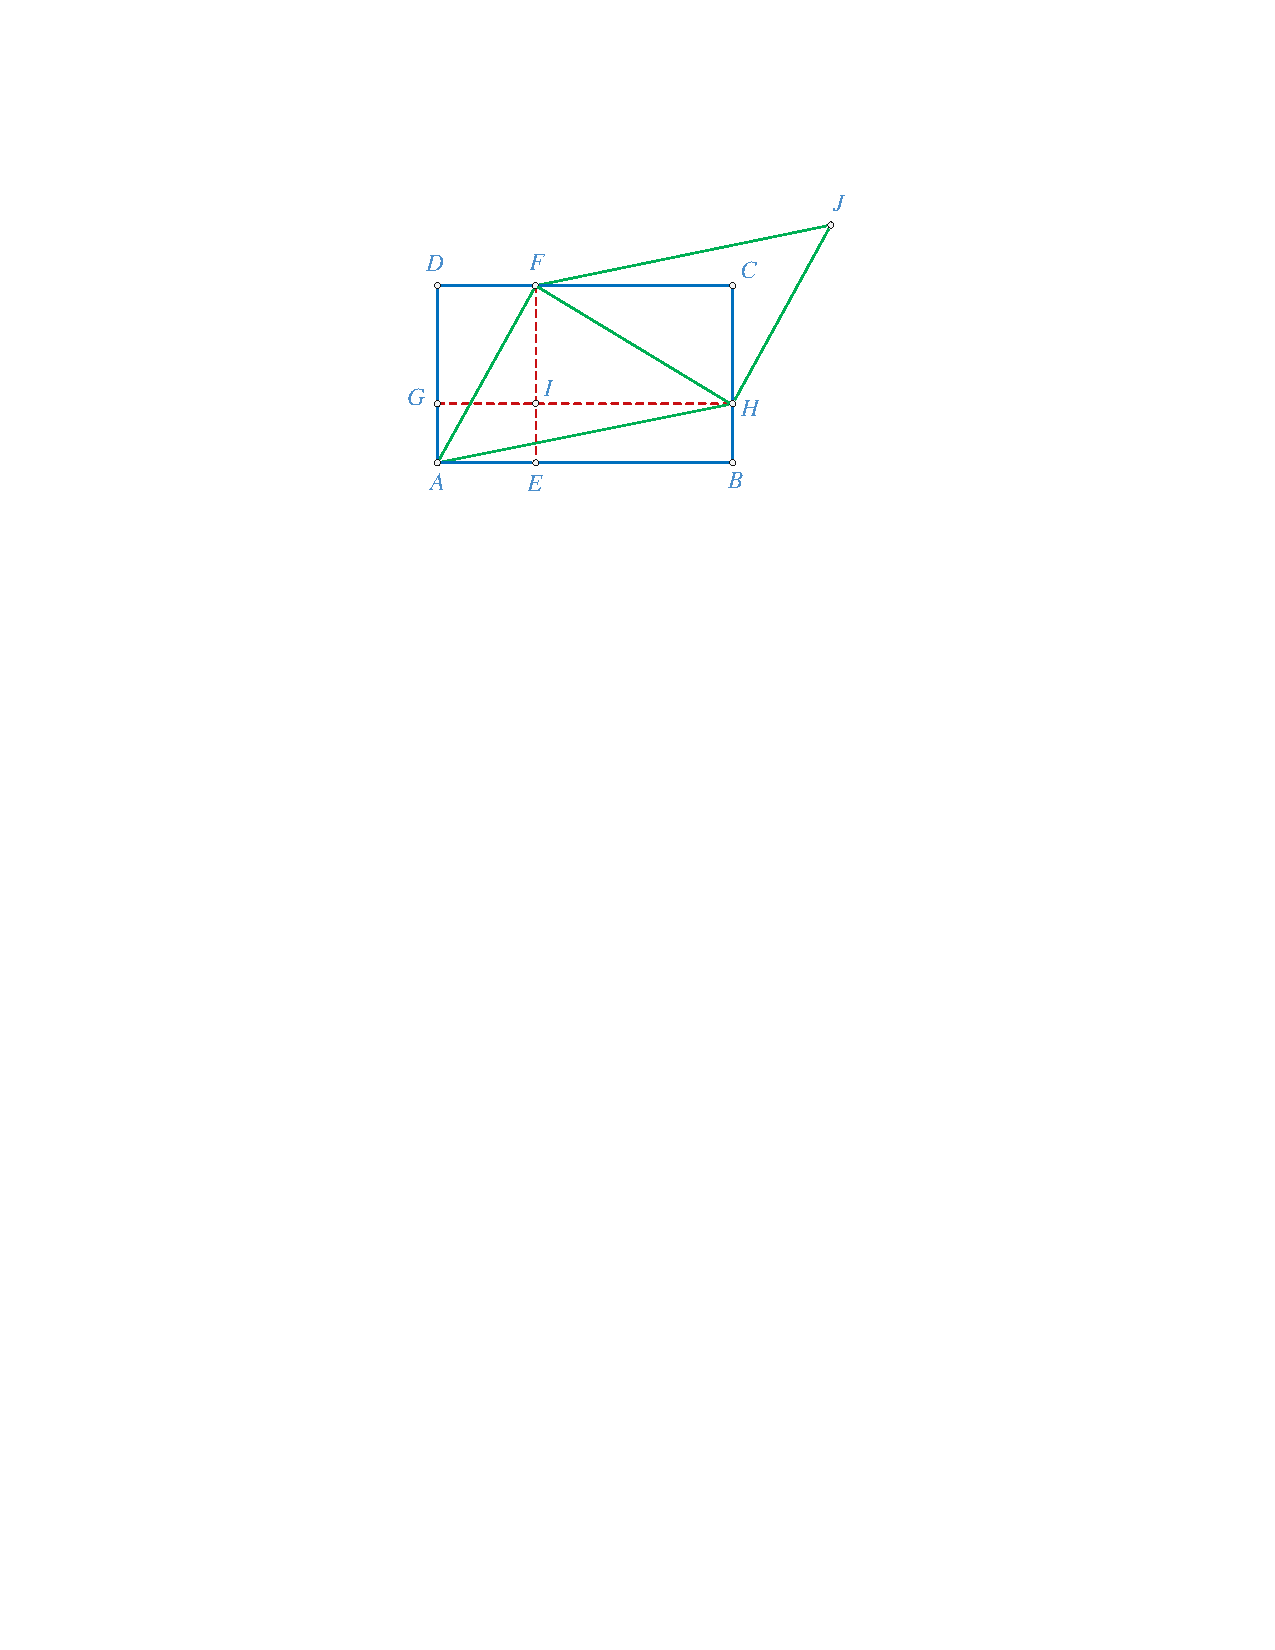
\includegraphics[width= 0.9\linewidth]{OC14}
		\vspace*{-15pt}
	\end{figure}
	\textit{Lời giải.} Do $S_{AHJF}=2S_{AHF},$ ta chỉ cần tính diện tích tam giác $AHF.$
	\vskip 0.1cm
	Trước tiên ta có
	\begin{align*}
		S_{GIFD}\times S_{EBHI} & = (IG \times IF ) \times (IE\times IH) \\[-0.5ex]
		&= (IG \times IE) \times (IF\times IH )\\[-0.5ex]
		&= S_{AEIG}\times S_{IHCF}.
	\end{align*} 
	Từ đó tính được $S_{GIFD}=\dfrac{36}{5}.$ Như vậy, ta biết diện tích hình vuông
	\begin{align*}
		S_{ABCD}=3+5+12+\frac{36}{5}=27\frac{1}{5}.
	\end{align*}
	Do đó, ta tính được
	\begin{align*}
		S_{AHF}&=S_{ABCD}-S_{AFD}-S_{FHC}-S_{ABH}\\[-0.5ex]
		&=S_{ABCD}-\frac{S_{AEFD}}{2}-\frac{S_{ABHG}}{2}-\frac{S_{IHCF}}{2}\\[-0.5ex]
		&= 27\frac{1}{5} - \frac{51}{10} - 4- 6= 12\frac{1}{10}.
	\end{align*}
	Như vậy diện tích hình bình hành $AHJF$ là $ 24\dfrac{1}{5}.$
	\vskip 0.1cm
	{\bf\color{cackithi} OC$\pmb{15.}$} Chúng ta xét các hàng ngang gồm $2020$ đồng tiền xu, mỗi đồng có mệnh giá $1$, $2$ hoặc $3$. Biết rằng :
	\vskip 0.1cm
	$\bullet$ Giữa hai đồng xu mệnh giá $1$ luôn có ít nhất một đồng xu khác;
	\vskip 0.1cm
	$\bullet$ Giữa hai đồng xu mệnh giá $2$ luôn có ít nhất hai đồng xu khác;
	\vskip 0.1cm
	$\bullet$ Giữa hai đồng xu mệnh giá $3$ luôn có ít nhất ba đồng xu khác.
	\vskip 0.1cm
	Hỏi có bao nhiêu hàng khác nhau gồm $2020$ đồng xu thỏa mãn các điều kiện trên?
	\vskip 0.1cm
	\textit{Lời giải.} Xét một dãy hàng ngang $2020$ thỏa mãn các điều kiện của bài toán. Tạm thời bỏ đi các đồng xu mệnh giá $3$ (nếu có) ra khỏi hàng, ta nhận được các dãy các đồng xu liên tiếp, mỗi đồng có mệnh giá $1$ hoặc $2$ (chúng được ngăn cách nhau bởi các đồng xu mệnh giá $3$ ban đầu).
	\vskip 0.1cm
	Nhận xét rằng một dãy các đồng xu liên tiếp như vậy (mỗi đồng có mệnh giá $1$ hoặc $2$) không chứa hai đồng mệnh giá $2$, vì nếu không khi đó, theo điều kiện thứ hai, giữa hai đồng mệnh giá $2$ liên tiếp có hai đồng mệnh giá $1$ đứng cạnh nhau, mâu thuẫn với diều kiện đầu tiên. Như vậy, một dãy liên tiếp các đồng xu mệnh giá nhỏ hơn $3$ chỉ có $5$ loại sau: 
	\begin{align*}
		121; 12; 21; 1; 2.
	\end{align*} 
	Mà theo điều kiện thứ ba, giữa hai đồng mệnh giá $3$ có đúng $3$ đồng xu khác, do đó trong $5$ loại trên thì $4$ loại sau không thể xuất hiện, nghĩa là giữa hai đồng mệnh giá $3$ liên tiếp có đúng $3$ đồng xu như sau: $31213.$ Vì vậy dãy $2020$ đồng xu thỏa mãn đề bài sẽ có dạng:
	\begin{align*}
		\underbrace{\cdots}_{\text{không chứa $3$}} \underbrace{312131213\cdots 31213}_{k \ \text{dãy}\ 3121\ \text{và thêm số} \ 3 } \underbrace{\cdots}_{\text{không chứa $3$}}.
	\end{align*}
	Do mỗi khúc ở đầu và cuối chứa không quá $3$ đồng xu nên chỉ có duy nhất một khả năng là $k=504$ và tổng số đồng xu ở cả hai khúc đầu và cuối bằng $3$. Ta có $10$ lựa chọn cho khúc đầu và cuối như sau:
	\begin{table}[H]
%		\vspace*{-5pt}
		\centering
		\captionsetup{labelformat= empty, justification=centering}
				\setlength{\tabcolsep}{5pt}
		\resizebox{\columnwidth}{!}{\begin{tabular}{|c|c|c|c|c|c|c|c|c|c|c|}
				\hline
				\makecell{Khúc\\đầu} & $\emptyset$ & $1$ & $1$ & $2$ & $2$ & $12$ & $12$ & $21$ & $21$ & $121$ \\
				\hline
				\makecell{Khúc\\cuối}	& $121$ & $12$ & $21$ & $12$ & $21$ & $1$ & $2$ & $1$ & $2$ & $\emptyset$ \\
				\hline
		\end{tabular}}
		\vspace*{-5pt}
	\end{table}
	Như vậy có $10$ hàng khác nhau gồm $2020$ đồng xu thỏa mãn đầu bài.
	\vskip 0.1cm
	Trong phần cuối của chuyên mục kỳ này, chúng tôi sẽ giới thiệu với bạn đọc ba bài toán trong kỳ thi Olympic Toán học Trẻ của Estonia năm học $2020-2021$. Các bài toán này phù hợp với trình độ học sinh Trung học cơ sở.
	\vskip 0.1cm
	{\bf\color{cackithi} OC$\pmb{22.}$} Tia phân giác tại đỉnh $A$ của tam giác $ABC$ cắt đường tròn ngoại tiếp tam giác $ABC$ tại điểm $F (F \neq A).$ Lấy điểm $D$ và $E$ lần lượt trên các cạnh $AB$ và $AC$ sao cho $DE$ song song với $BC$. Gọi $G$ và $H$ lần lượt là giao điểm của các tia $FD$ và $FE$ với đường tròn ngoại tiếp tam giác $ABC (G \neq F, H \neq F).$ Các đường tròn ngoại tiếp tam giác $AGD$ và $AHE$ cắt nhau tại điểm $P (P \neq A).$ Chứng minh rằng điểm $P$ nằm trên đường thẳng $AF$.
	\begin{figure}[H]
		\vspace*{-10pt}
		\centering
		\captionsetup{labelformat= empty, justification=centering}
		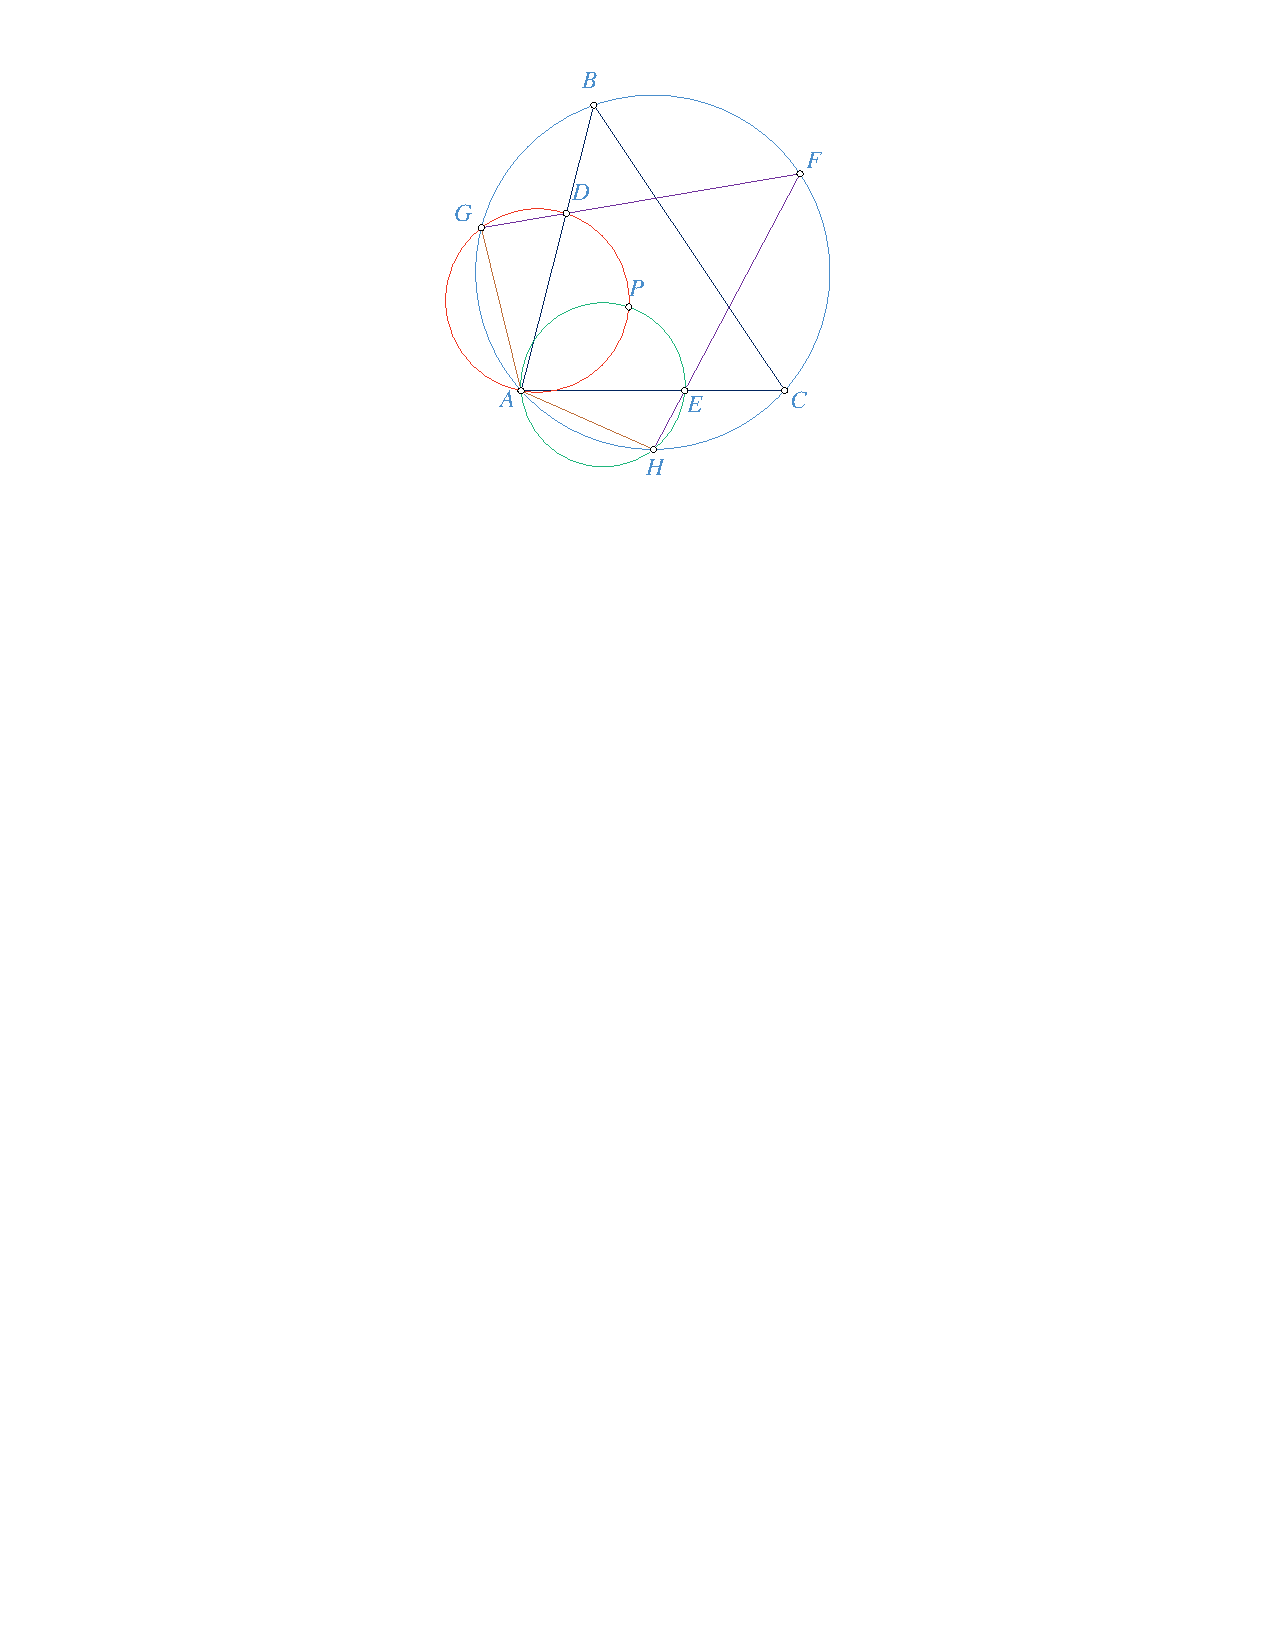
\includegraphics[width= 0.8\linewidth]{OC22}
		\vspace*{-10pt}
	\end{figure}
	{\bf\color{cackithi} OC$\pmb{23.}$} Tìm tất cả các số nguyên $n\ge 3$ sao cho có thể viết một số
	(không nhất thiết là số nguyên) vào mỗi đỉnh của một đa giác đều $n$ cạnh thỏa mãn cả hai điều kiện sau:
	\vskip 0.1cm
	$(1)$  Với bất kỳ ba đỉnh liên tiếp theo chiều kim đồng hồ của đa giác, 
	chứa các số $x, y$ và $z$ tương ứng, thì ta có $x=|y-z|$;
	\vskip 0.1cm
	$(2)$ Tổng các số trong tất cả các đỉnh của đa giác bằng $1$.
	\vskip 0.1cm
	{\bf\color{cackithi} OC$\pmb{24.}$} Có một bộ $8$ quân cờ domino như trong hình vẽ bên dưới, mỗi quân gồm hai ô vuông đơn vị:
	\begin{figure}[H]
		\vspace*{-5pt}
		\centering
		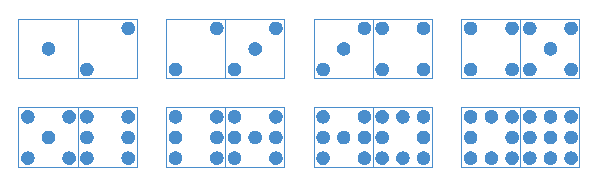
\includegraphics[width=0.9\linewidth]{OC24}
		\vspace*{-10pt}
	\end{figure}
	Liệu có thể lát kín hoàn toàn một bảng vuông có kích thước $4 \times 4$ bằng những quân domino này sao cho tổng số chấm trên mỗi hàng, mỗi cột đều bằng nhau?
\end{multicols}

